\documentclass[letterpaper, 11pt]{article}
\usepackage[margin=1in]{geometry}
\usepackage{graphicx}
\usepackage{amssymb}
\usepackage{amsmath}
\usepackage{epstopdf}
\usepackage{url}
\usepackage{hyperref}

\title{CS175 - Assignment 2 \\Playing with Frames (on paper)}
\date{}

\begin{document}
\maketitle

\textbf{Completed by: Emily Sun + Lauren (PK) Byunn-Rieder}\\


Do exercises 4.1, 4.2, 4.3, and 4.4 from the book. These are given here
in a companion file, and so you do not need the book.

Your written submission can be in txt, doc(x), odt, or pdf format. Submit using Canvas. For problems requiring
a figure, you need to submit the figure somehow (embedded in the
doc/odt/pdf, or as an additional image file).

Explain your reasoning.

\subsection*{Notes:}

\begin{itemize}
\item \textbf{4.1:} Regarding ``definitions of section 4.2'' all you need to know is that
$R$ is a $45$-degree rotation counter clockwise, and $T$ is a
positive translation  along the first axis.

You should have images interpreting the transformation left-to-right and images interpreting the transformation right-to-left.\\

\fbox{%
  \begin{minipage}{6in}
The transformation left to right is a local transformation where we first rotate the frame, then transform it by moving along the rotated frame's first axis. Shown below:
  \end{minipage}%
}


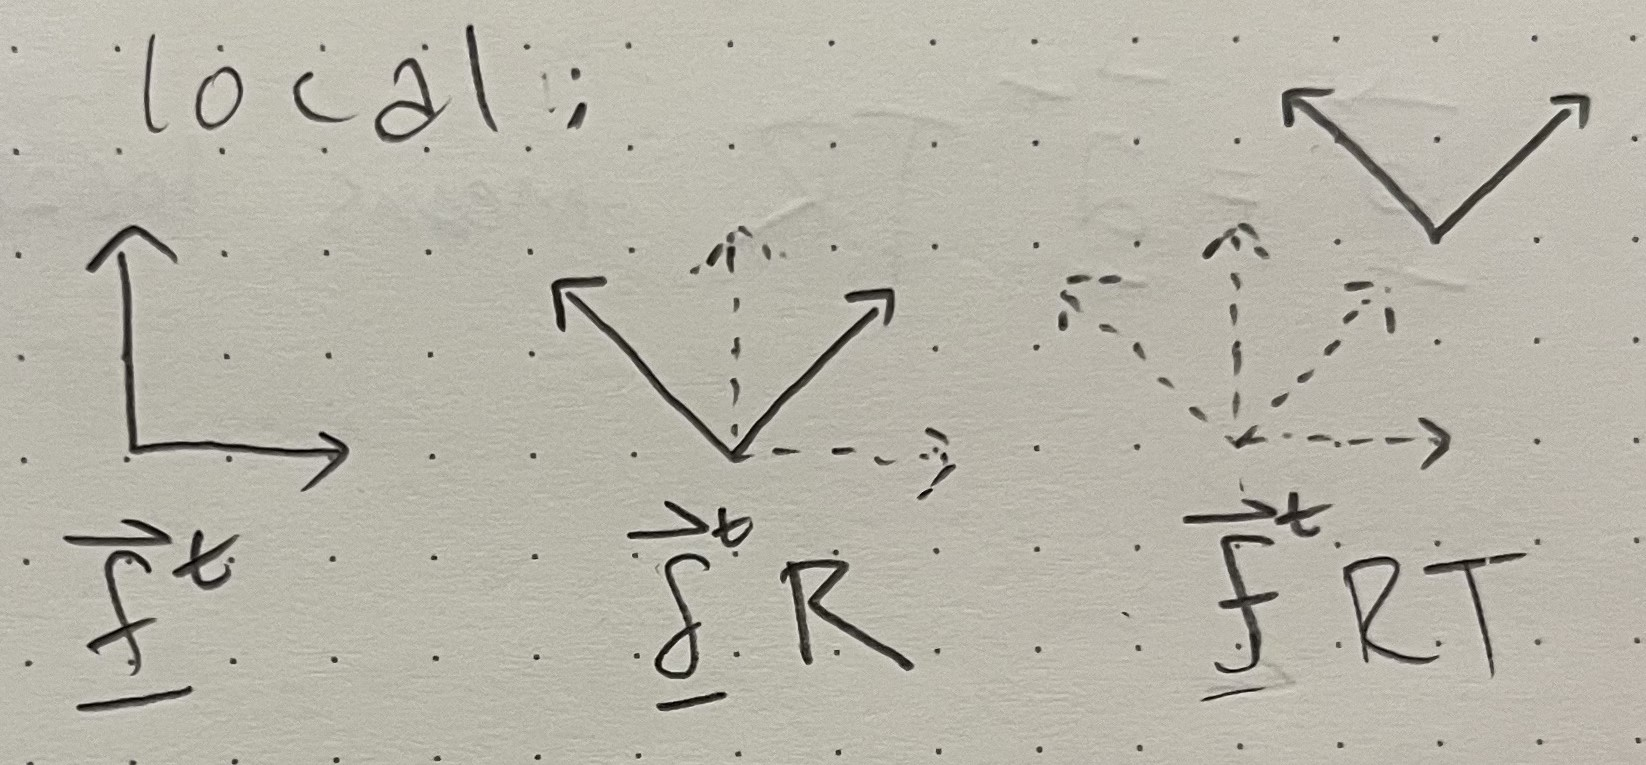
\includegraphics[width=0.87\textwidth]{1.jpg}

\fbox{%
  \begin{minipage}{6in}
The transformation right to left is a global transformation where we first transform the frame by moving it along the first axis, then rotate about the origin of the original frame. Shown below:
   \end{minipage}%
}


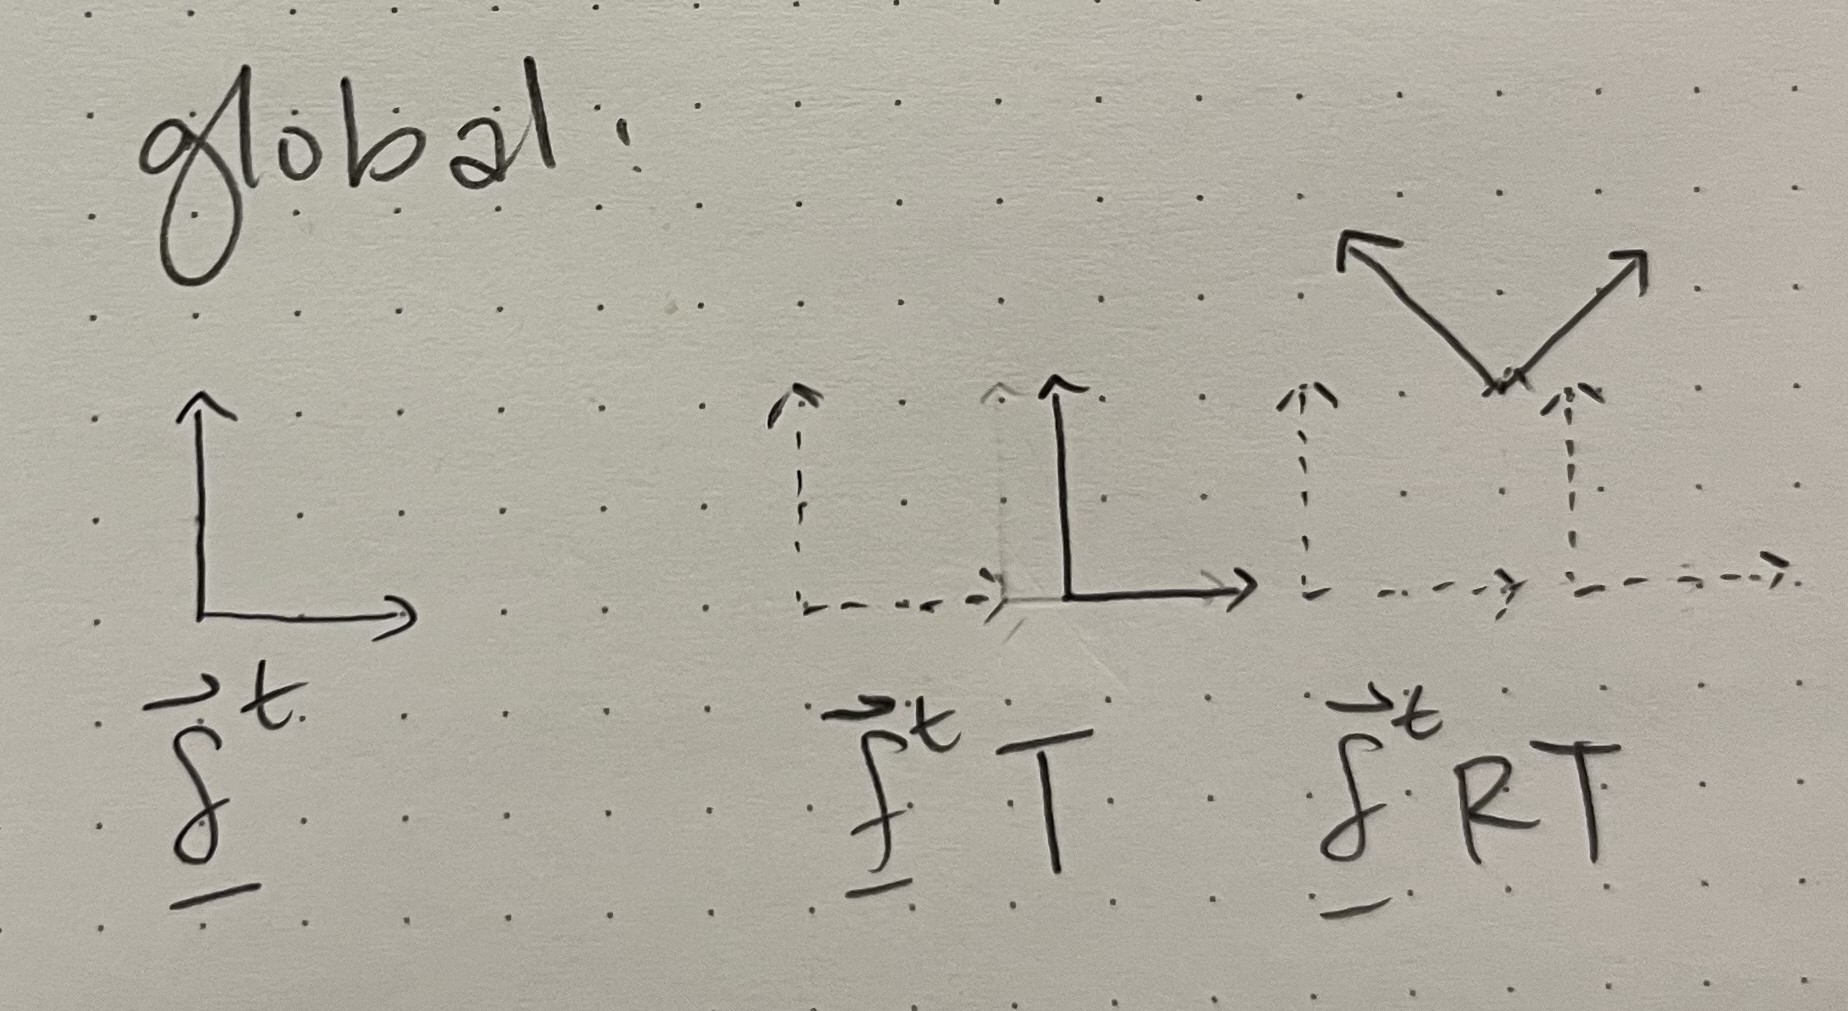
\includegraphics[width=0.87\textwidth]{2.jpg}

\item \textbf{4.2:} Note that the transformation specified here is different from the one shown in lecture.
  Just to be clear, in 2D,
  the matrix $T$ is a matrix
  with rightmost column is $[1,0,1]^t$.\\

\fbox{%
  \begin{minipage}{6in}
The origin of the frame moves two of the original frame's units. Reading left-to-right, we first scale the frame two times larger, then translate by one unit of the scaled frame, which is equivalent to two units of the original frame. Thus, the origin of the frame moves by 2f along the x-axis.

  \end{minipage}%
}


\item \textbf{4.3:} You don't need to write out what is in the rotation matrix. You can
just write $R_\theta$.  This question has two parts!

\fbox{%
  \begin{minipage}{6in}
In \textbf{both} cases, the rotation matrix is
\[ R = 
\begin{bmatrix}
    R_\theta & 0 \\
    0 & 1
\end{bmatrix}
\]

For $\vec{\textbf{b}}^t = \vec{\textbf{a}}^t T R$, the translation matrix represents moving $d_1$ in $\vec{\textbf{a}}^t$'s first axis and $d_2$ in its second:
\[ T = 
\begin{bmatrix}
    1 & 0 & d_1 \\
    0 & 1 & d_2 \\
    0 & 0 & 1
\end{bmatrix}
\]

For $\vec{\textbf{b}}^t = \vec{\textbf{a}}^t R T$, the translation matrix represents moving $d_3$ in $\vec{\textbf{a}}^t R$'s first axis and $d_3$ in its second:

\[ T = 
\begin{bmatrix}
    1 & 0 & d_3 \\
    0 & 1 & d_4 \\
    0 & 0 & 1
\end{bmatrix}
\]

\end{minipage}
}

\item \textbf{4.4:} This is a bit tricky. First of all, the orange point is not
necessarily along the first black axis. Second of all, I do not want to
see $d$ or $\phi$ in the answer. All you need to know is that both thin black lines have the same length ($d$), and make the same angles ($\phi$) with the appropriate frames.

Think about what you physically ``do'' to  transform the black to become the orange frame.

\fbox{%
  \begin{minipage}{6in}

The transformation from the black frame $\vec{\textbf{a}}^t$ to the orange frame $\vec{\textbf{c}}^t$ can be thought of as a rotation of $\theta$ about the origin of the blue frame $\vec{\textbf{b}}^t$. So we know two things: $\vec{\textbf{c}}^t = \vec{\textbf{a}}^t M$ and $\vec{\textbf{c}}^t = \vec{\textbf{a}}^t$ rotated by $\theta$ with respect to $\vec{\textbf{b}}^t$. Therefore we know that the matrix $M$ is the same as the matrix that rotates by $\theta$ with respect to $\vec{\textbf{b}}^t$.

We'll start with $\vec{\textbf{a}}^t$ and transform it. $\vec{\textbf{b}}^t = \vec{\textbf{a}}^tN$ is equivalent to $\vec{\textbf{a}}^t = \vec{\textbf{b}}^t N^{-1}$ if we rearrange.

$$\vec{\textbf{a}}^t = \vec{\textbf{b}}^t N^{-1}$$

Now we have it in a nice format to use the left-of rule because we want to rotate with respect to $\vec{\textbf{b}}^t$. To do this transformation, we'll add a rotation matrix $R_\theta$ immediately to the right of $\vec{\textbf{b}}^t$:

$$\rightarrow \vec{\textbf{b}}^t R_\theta N^{-1}$$

Then we can put it back in terms of $\vec{\textbf{a}}^t$ because we know the relation between $\vec{\textbf{a}}^t$ and $\vec{\textbf{b}}^t$:

$$= \vec{\textbf{a}}^t N R_\theta N^{-1}$$

Since this represents $\vec{\textbf{a}}^t$ rotated by $\theta$ about $\vec{\textbf{b}}^t$, this is $\vec{\textbf{c}}^t$. So we have two true statements:

$$\vec{\textbf{c}}^t = \vec{\textbf{a}}^t N R_\theta N^{-1}$$
$$\vec{\textbf{c}}^t = \vec{\textbf{a}}^t M$$

which then easily shows that
$$M = N R_\theta N^{-1}$$

We can also expand what $R_\theta$ is exactly. We know that it's a counter-clockwise rotation by $\theta$, so we can express it with trigonometric terms:

\[ R_\theta = 
\begin{bmatrix}
    \cos(\theta) & -\sin(\theta) & 0 \\
    \sin(\theta) & \cos(\theta) & 0 \\
    0 & 0 & 1
\end{bmatrix}
\]

All together, that means

\[M = N \begin{bmatrix}
    \cos(\theta) & -\sin(\theta) & 0 \\
    \sin(\theta) & \cos(\theta) & 0 \\
    0 & 0 & 1
\end{bmatrix} N^{-1}\]

   \end{minipage}%
}

\end{itemize}

\end{document}
